\chapter{Literature Review}\label{chapter:2}

\section{Overview of Low Earth Orbit Satellite Communications}
%LEo satellite communications 

\section{LEO Satellite Constellation Architectures}
% Describes common constellation designs, orbital shells,
% inclinations, and scaling considerations.

\section{Existing LEO Constellations}
% Reviews major operational and planned LEO systems
% such as Starlink, OneWeb, and Telesat.

\section{Coverage and Latency Characteristics of LEO Systems}
% Discusses global coverage potential and latency advantages
% of LEO satellites relative to other orbit classes.

\section{Capacity and Throughput Modelling in Satellite Networks}
% Reviews literature on bandwidth allocation, beam usage,
% and throughput limitations in satellite systems.

\section{Integration of LEO Satellites with Mobile carriers}
% Examines hybrid satellite--terrestrial network models,
% backhaul use cases, and coexistence with fibre and wireless systems.

\section{Challenges and Limitations of LEO Systems}
% Covers orbital congestion, spectrum regulation,
% system complexity, and sustainability issues.




\section{LEO Satellite Coverage Analysis in Other Countries}
Several countries with with large rural or remote populations have adopted LEO satellite communications to provide broadband access where terrestrial networks are economically feasible. 



\subsection{Canada}
In Canada, LEO satellites have been used to address broadband deficiencies, in northern and remote regions. Both Starlink and OneWeb have been deployed to provide last-mile connectivity or satellite back-haul to local wireless networks. Government-backed initiatives have supported the integration of LEO services to complement terrestrial infrastructures, recognizing how they can lower latency and higher capacity over traditional satellite and terrestrial links. Canadian studies show that LEO systems offer a cost effective alternative \cite{telesat_canada_leo_2026}. 

\subsection{Australia}
Australia has formally integrated LEO broadband into its national broadband strategy. In 2025, the government owned National Broadband Network (NBN) annoyed a transition from geostationary satellites to LEO satellites for regional and remote users in partnership with Amazons Kuiper. The goal of this is to provide a lower latency and higher quality broadband to rural and remote premises number over 300,000. This use case shows LEO satellites can provide broadband performance close to terrestrial services, particularly in rural areas \cite{nbn_kuiper_2025}. 

\subsection{United States of America - Alaska}



Alaska has one of the most well developed deployments of LEO satellite broadband. Due to the rugged geography, low population density and permafrost conditions, fibre deployment is exceptionally expensive and challenging in many regions. As a result, large areas of rural Alaska have historically relied on geostationary satellite systems or low-capacity legacy connections, which offer limited performance and high latency.

In recent years, LEo satellite systems - primarily Starlink - have been adopted across rural Alaskan communities. These services are being used by households as well as public institutes such as schools, healthcare facilities, and emergency services. Deployment reports show that LEO broadband has enabled reliable internet, with government funded programmes which incorporate LEO services for undeserved regions\cite{aasb_starlink_alaska}.

Independent performance measurement analyses further shows the benefits of LEO systems in Alaska. COmpared to traditional Geostationary services, LEO connectivity has been shown to significantly reduce latency and improve overall service reliability. LEO broadband now form a core component of Alaska's broadband strategies, with government funded programmes incorporating LEO services. \cite{ookla_alaska_connectivity_2026}

Alaska is set to receive \$1.2 billion in funding from the federal government's Broadband Equity Access and Deployment (BEAD) program, of which \$629 million has been set aside for broadband projects. This will be used to connect 44,734 under-served or unserved locations across Alaska. Due to the previously discussed geography issues, this initiative will use a mix of technologies. 14,400 of these locations will be served with Starlink. A breakdown of how this broadband will be rolled out can be seen in Figure \ref{fig:AlaskaBEAD}.

\begin{figure}[htbp]
    \centering
    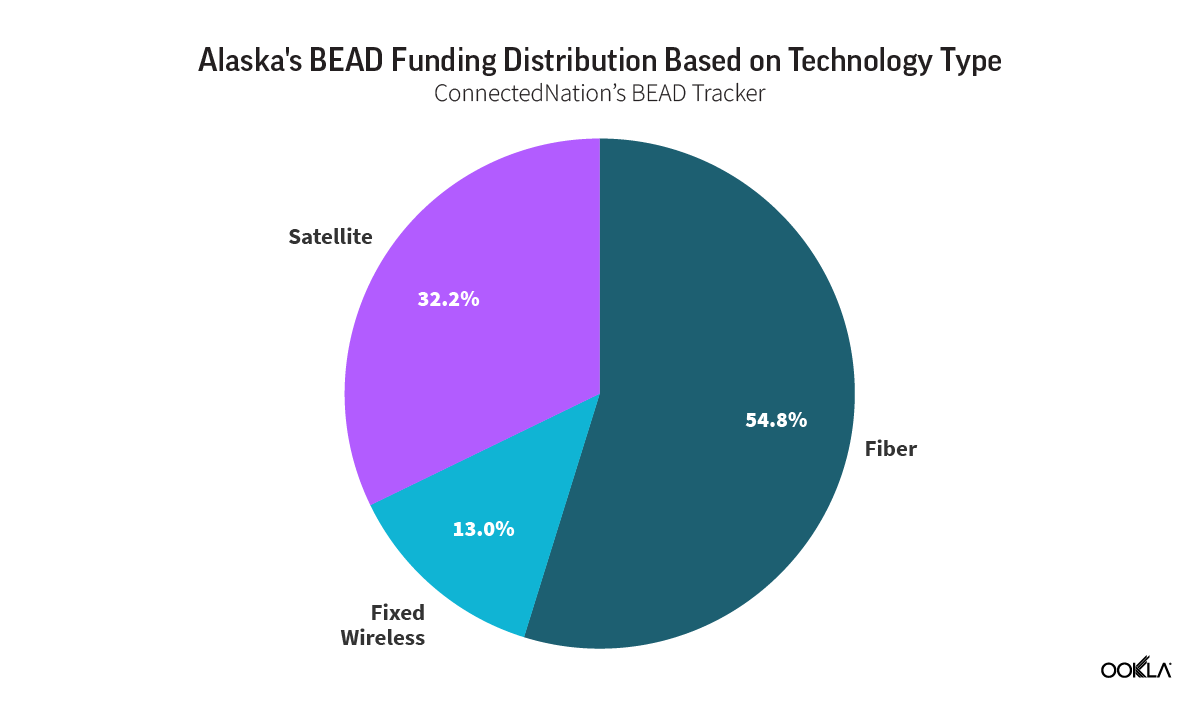
\includegraphics[width=0.6\textwidth]{figures/Alaska_broadband_budget.png}
    \caption{Alaska's BEAD Funding and Distribution Based on Technology Type \cite{ookla_alaska_connectivity_2026}}
    \label{fig:AlaskaBEAD}
\end{figure}
\FloatBarrier

Starlink in 2025 was able to bring up the percentage of Ookla speedtest users in Alaska with broadband speeds of 100/20  Mbps from $4.35\%$ in the first half of 2025 to $15.9\%$ in the second half of 2025. In fact a greater number of rural Starlink users in Alaska are receiving broadband speeds of 100/20 Mbps than it's urban users. By the end of 2025 $16.8\%$ of Starlink users in rural areas were able to get broadband speeds of 100/20 Mbps compared to just $12.3\%$ of urban users \cite{ookla_alaska_connectivity_2026}.

According to Ookla, Starlink's median download speeds rose from 73.5 Mbps in March 2025 to 108.5 Mbps in March 2026, and it's median upload speeds go from 10.7 Mbps in March 2025 to 17.1 Mbps in March 2026. This increase in speed can be seen in Figures \ref{fig:alaska_downspeed} and \ref{fig:alaska_upspeed}.


\begin{figure}[htbp]
  \centering
  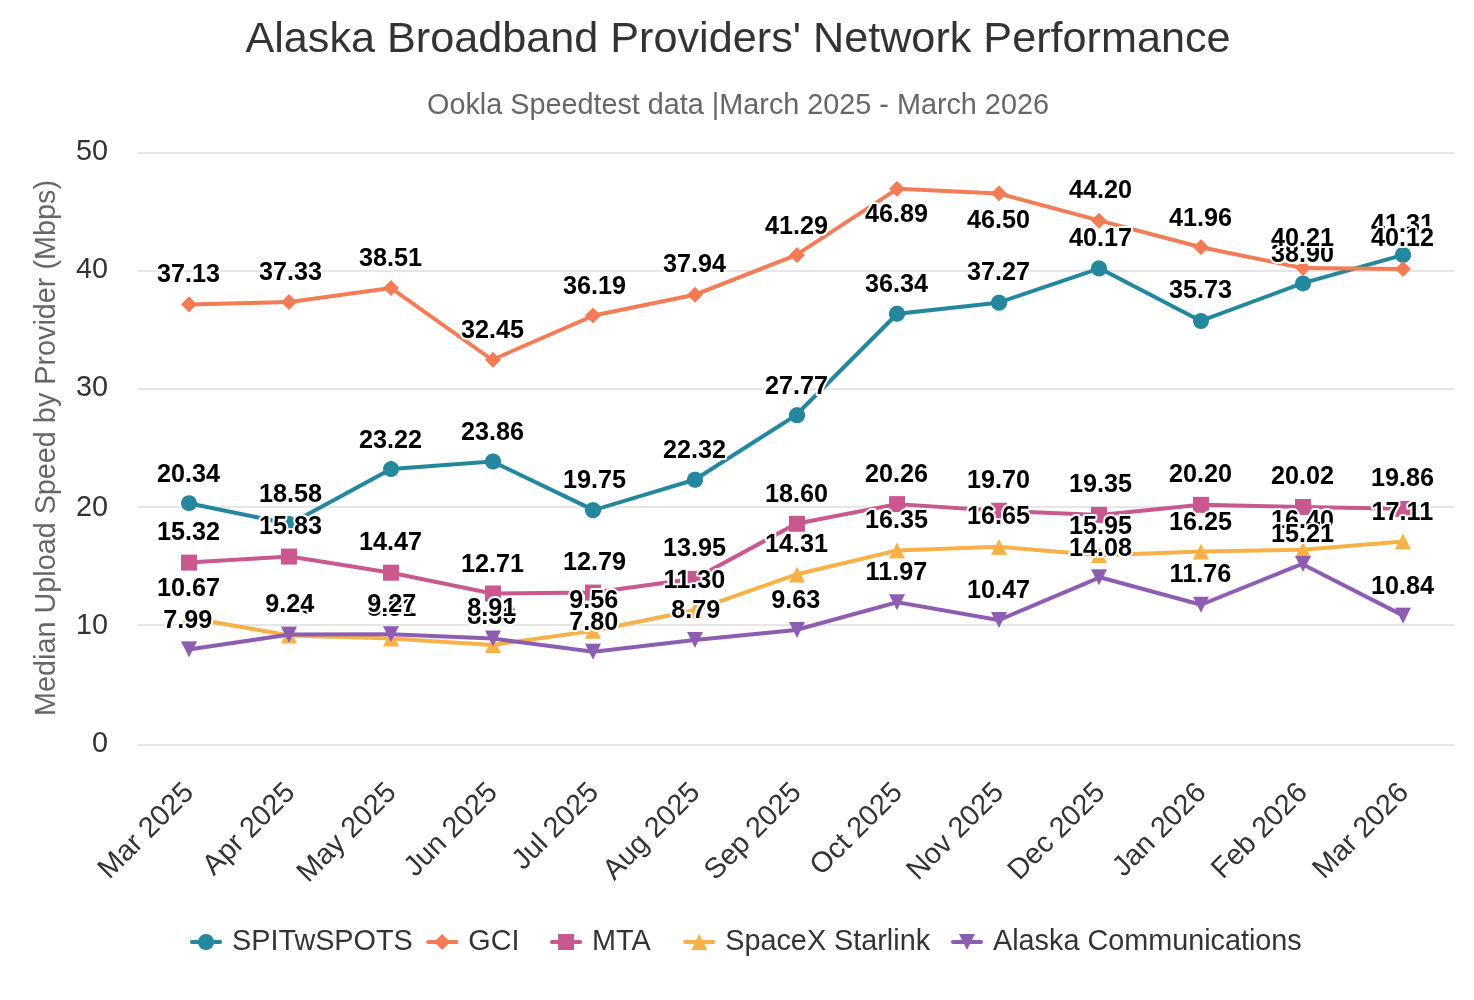
\includegraphics[height=0.4\textheight]{figures/alaska-broadband-provide.png}
  \caption{Alaska broadband plot of downlink speeds.}
  \label{fig:alaska_downspeed}
\end{figure}

\begin{figure}[htbp]
  \centering
  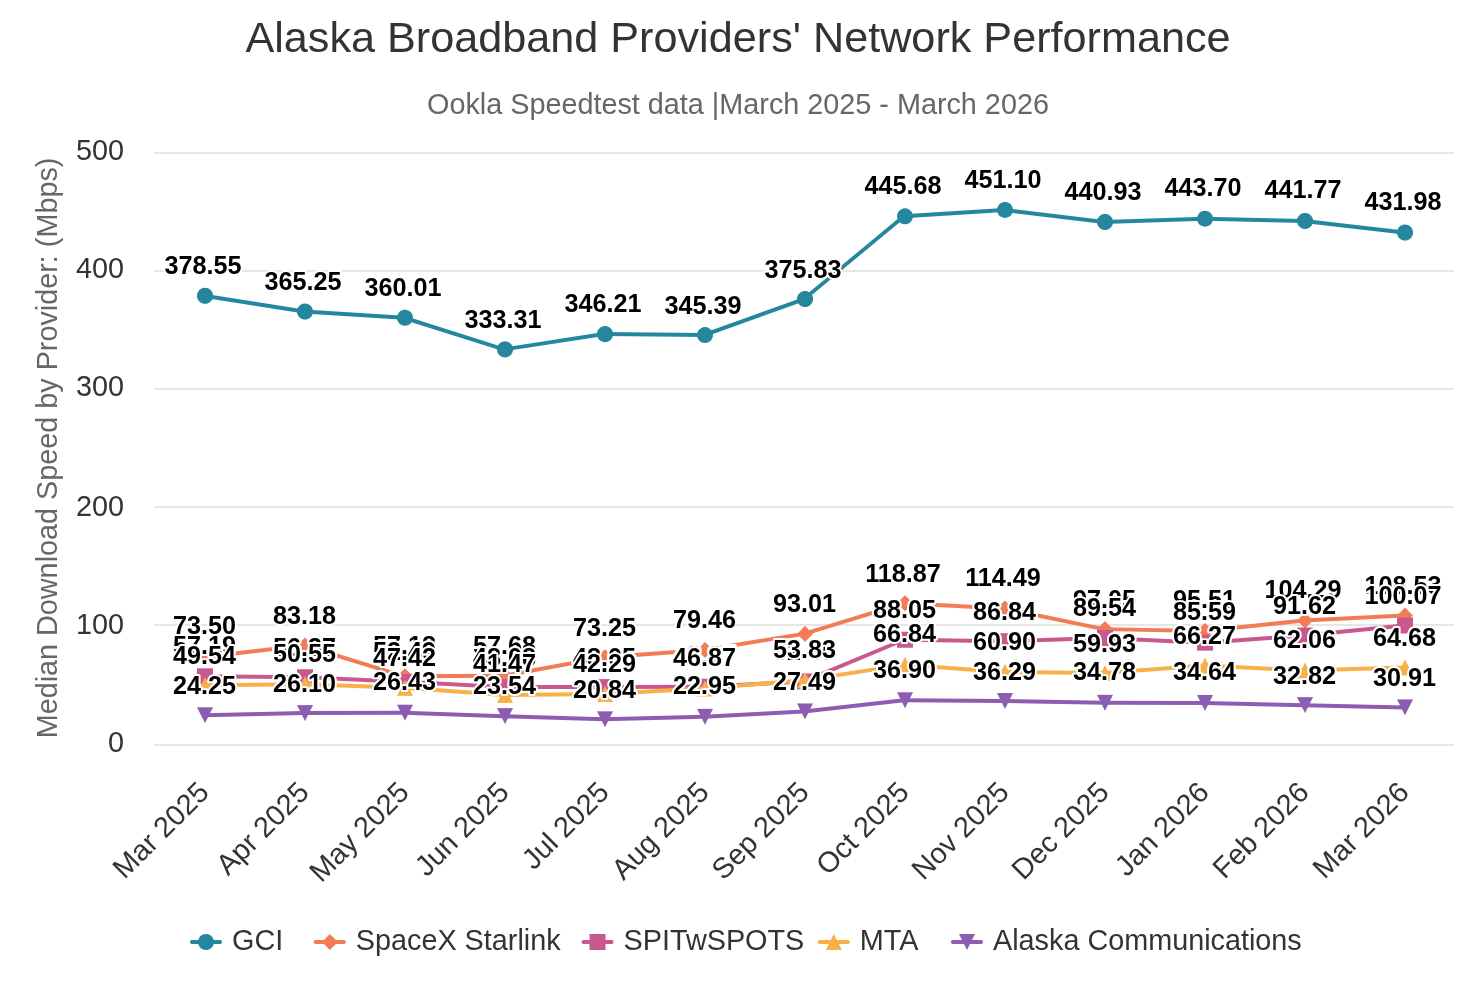
\includegraphics[height=0.4\textheight]{figures/alaska-broadband-provide (1).png}
  \caption{Alaska broadband plot of uplink speeds.}
  \label{fig:alaska_upspeed}
\end{figure}

\FloatBarrier

This provides solid evidence of a real world example of how LEO satellite broadband can function as along term connectivity solution. While there are differences in Ireland such as environmental differences, the underlying challenges are the same - low population density, high infrastructure costs, and limited commercial incentives for fibre deployment. Alaska is a compelling case to further investigate the potential for LEO broadband in Ireland. 

\subsection{Relevance to Ireland}
These international examples demonstrate that LEO constellations are increasingly becoming a viable option for providing broadband in rural areas. Common across all cases are low population density, and challenging geography with high costs for terrestrial network deployment. These conditions align closely with what can be found in regions in Ireland.  




\section{LEO Satellite Upgrading}
% Discusses satellite replacement cycles and constellation evolution.

\section{Future Trends in LEO Satellite Communications}
% Explores emerging trends such as NTN integration,
% 6G compatibility, and next-generation LEO systems.

\section{Summary and Research Gap}
% Synthesises the literature and identifies the gap
% addressed by this thesis.

